\documentclass[compress]{beamer}
\usepackage[utf8]{inputenc}
\usepackage[francais]{babel}
\usepackage[T1]{fontenc}
\usepackage{amssymb}
\usepackage{amsmath}
\usepackage{amsfonts}
\usepackage{hyperref}
\usepackage[]{algorithm2e}
\usepackage{amssymb}
\usepackage{verbatim}
\usepackage{listings}
\usepackage{color}
\usepackage{graphicx}
\usepackage{subfig}
\usetheme[navigation]{UMONS}

\author{Benjamin André, Alexis Lecocq}
\title{Statistiques multidimensionnelles}
\subtitle[\ldots]{Réseaux de neurones (NN)}

\setbeamercovered{transparent} 
\setbeamertemplate{navigation symbols}{} 
\institute{UMONS\\Faculté des Sciences\\BA 3 Sciences Informatiques\\[2ex]
  
\includegraphics[height=4ex]{UMONS}\hspace{2em}%
  \raisebox{-1ex}{
\includegraphics[height=6ex]{UMONS_FS}}}
\date{Juin 2017} 
\definecolor{darkgreen}{rgb}{0.0, 0.2, 0.13}
\subject{Statistiques multidimensionnelles} 
\lstset{ %
  language=R,                     % the language of the code
  basicstyle=\footnotesize,       % the size of the fonts that are used for the code
  numbers=left,                   % where to put the line-numbers
  numberstyle=\tiny\color{gray},  % the style that is used for the line-numbers
  stepnumber=1,                   % the step between two line-numbers. If it's 1, each line
                                  % will be numbered
  numbersep=5pt,                  % how far the line-numbers are from the code
  backgroundcolor=\color{white},  % choose the background color. You must add \usepackage{color}
  showspaces=false,               % show spaces adding particular underscores
  showstringspaces=false,         % underline spaces within strings
  showtabs=false,                 % show tabs within strings adding particular underscores
  frame=single,                   % adds a frame around the code
  rulecolor=\color{black},        % if not set, the frame-color may be changed on line-breaks within not-black text (e.g. commens (green here))
  tabsize=2,                      % sets default tabsize to 2 spaces
  captionpos=b,                   % sets the caption-position to bottom
  breaklines=true,                % sets automatic line breaking
  breakatwhitespace=false,        % sets if automatic breaks should only happen at whitespace
  title=\lstname,                 % show the filename of files included with \lstinputlisting;
                                  % also try caption instead of title
  keywordstyle=\color{blue},      % keyword style
  commentstyle=\color{darkgreen},   % comment style
  stringstyle=\color{violet},      % string literal style
  escapeinside={\%*}{*)},         % if you want to add a comment within your code
  morekeywords={*,...}            % if you want to add more keywords to the set
} 

\begin{document}

	\begin{frame}
		\titlepage
	\end{frame}

	\begin{frame}
		\tableofcontents
	\end{frame}

	
	\begin{comment}
		
		Structure du rapport de flo et clément
	
		\section{Description de CART}
		\subsection{Introduction}
		\frametitle{Définition}
		\subsection{Algorithme de construction le l'arbre 	CART}
		\frametitle{Comment l'arbre est-il construit ?}
		\frametitle{Exemple sur le jeu de données Titanic 	fourni avec R}	
		\section{Implémentation dans R}
		\frametitle{Introduction}
		\frametitle{Jeu de données}
		\frametitle{Création de l'arbre}
		\frametitle{Arbre final}
		\frametitle{Vérification du choix des tests}	
		\frametitle{Prédiction de la valeur d'une variable}
	\end{comment}

	\section{Description de NN}
		\subsection{Machine Learning}
			\begin{frame}
				\frametitle{Machine Learning}
				Lorsque nous voulons résoudre un problème algorithmiquement, nous devons donner la marche à suivre exacte du programme qui mène à une solution.
				
				Dans certains cas, celle-ci est trop complexe que pour être écrite de cette façon, et les paramètres d'entrée (position, température, couleur,..) peuvent influencer le résultat de façon très complexe.
				
				L'approche du machine learning propose de trouver une solution approchée en minimisant l'erreur.
			\end{frame}
			
			\begin{frame}
				\frametitle{Machine Learning}
				\begin{alertblock}{Utilisation}
					Comme expliqué précédemment, il s'agit d'une solution approchée. Dans le cas ou il existe un algorithme efficace il sera préférable de l'utiliser
				\end{alertblock}
				
				\begin{block}{Exemples}
					\begin{itemize}
						\item AlphaGo
						\item DeepBlue
						\item Voitures autonomes
						\item Filtre à spam
						\item Reconnaissance d'image
						\item Traduction
						\item Prévision de la bourse
					\end{itemize}
				\end{block}
			\end{frame}
		\subsection{Neural Networks (NN)}
			\begin{frame}
				\frametitle{Neural Networks}		
				\hspace{3em}%
				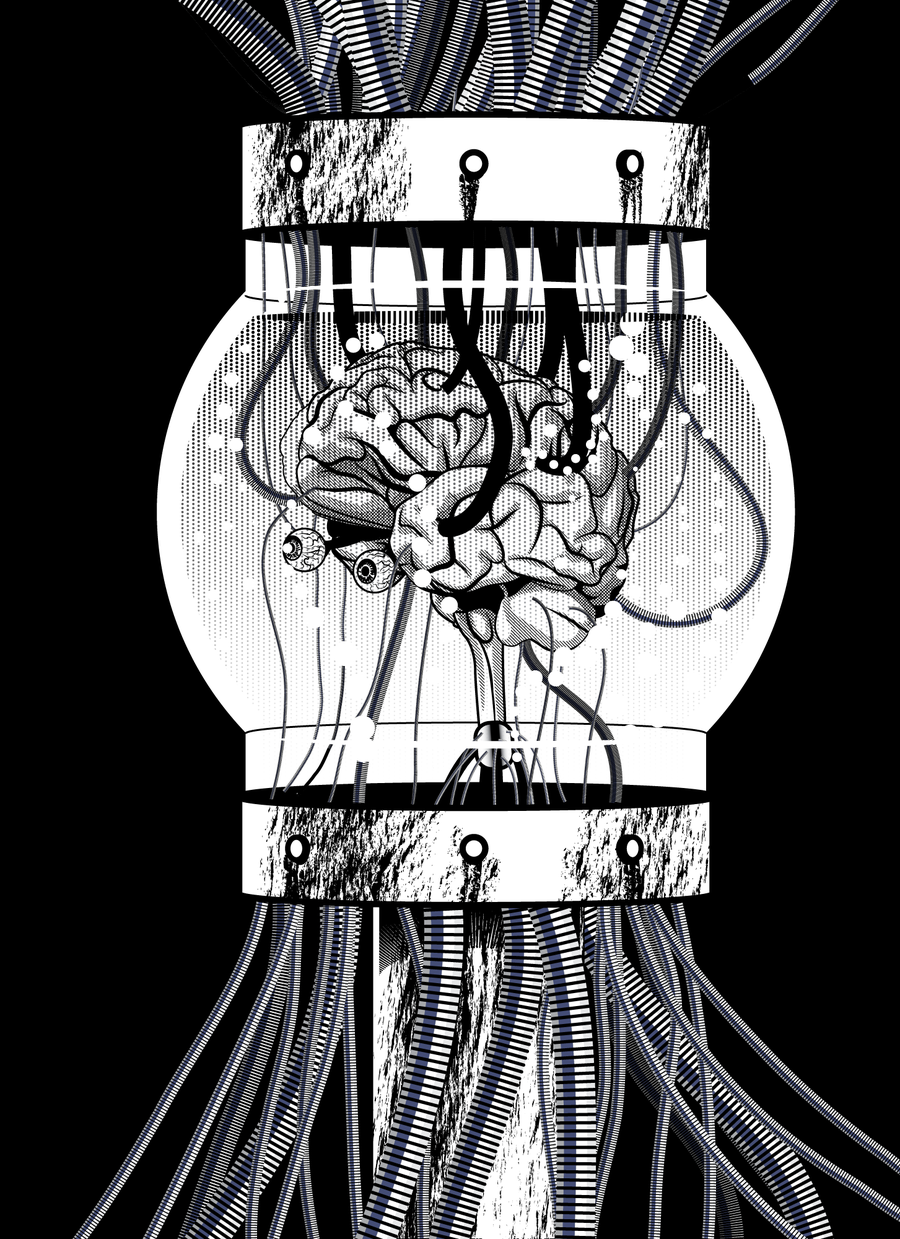
\includegraphics[height=100px]{img/brain}\hspace{2em}%
				\raisebox{-1ex}{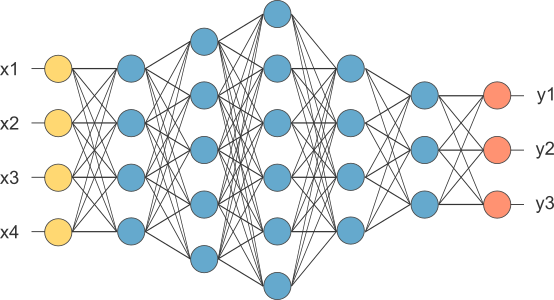
\includegraphics[height=100px]{img/deep_neural_network}}
				
				%Et ici on fait la blague qu'on pourrait penser au cerveau connecté et que ça fait peur, mais qu'en réalité... ça fait encore plus peur !
			\end{frame}


\section*{Sources}
\begin{frame}
\frametitle{Sources}
\url{https://www.r-bloggers.com/fitting-a-neural-network-in-r-neuralnet-package/}\\
\url{http://www.parallelr.com/r-deep-neural-network-from-scratch/}\\
\url{https://www.youtube.com/watch?v=BR9h47Jtqyw}\\
\url{http://doctor-morbius.deviantart.com/}\\
\url{https://datascienceplus.com/fitting-neural-network-in-r/}%d'ou on tient le code !
\end{frame}

\end{document}